\documentclass[UTF8,a4paper]{ctexart}
\usepackage{xcolor}
\usepackage{graphicx}
\usepackage[margin=1.5in]{geometry}
\usepackage{float}
\usepackage{listings} 
\usepackage{fancyhdr} %用于调整页眉的样式
\usepackage{fancyvrb} 
\usepackage{tabularx}
\usepackage[colorlinks,linkcolor=blue]{hyperref}%用于插入超链接
\usepackage{wallpaper}
\usepackage{tikz}
\usepackage{lipsum}
\usepackage{rotating}
\usepackage[absolute]{textpos}
\usetikzlibrary{calc}
\setlength{\TPHorizModule}{1cm}
\setlength{\TPVertModule}{1cm}



\definecolor{color1}{RGB}{10,80,179}
\pagestyle{fancy}
\fancyhead[L]{ }
\setlength{\headheight}{27pt}

\definecolor{GradientTop}{RGB}{0,0,255}
\definecolor{GradientBottom}{RGB}{255,0,0}
\colorlet{GradientMid}{blue!50!red}

\lstset{
    numbers=left,
    numberstyle=\tiny,
    frame=shadowbox,
    rulesepcolor= \color{ red!20!green!20!blue!20},
    escapeinside=``,
    xleftmargin=2em,aboveskip=1em,
    framexleftmargin=2em,
    breaklines=true
}

\hypersetup{
    colorlinks=true,            % 激活链接颜色,去掉链接边框
    urlcolor=color1           % 外部URL链接颜色
}

\begin{document}
%封面
\ThisCenterWallPaper{1.02}{background.png} 
\begin{textblock}{5}(1,2)
    % 设置字号为20pt
    \fontsize{15}{24}\selectfont
    \color{white}
    \begin{turn}{270}
         \qquad 取则行远
        \end{turn}
        \begin{turn}{270}
            海纳百川 
            \end{turn}
    
    \end{textblock}
\begin{center}
    %logo
    \begin{tikzpicture}[remember picture, overlay]
        % 绘制一个矩形,并设置其位置在页面的右上角
        \draw[fill=blue] (current page.north east) rectangle (current page.north west);
        % 在矩形中插入图片,并设置与右上角的距离
        \node[anchor=north east, xshift=-1cm, yshift=-2cm] at (current page.north east) {
            
\includegraphics[width=6cm]{logo.png}
        };
    \end{tikzpicture}

\begin{textblock}{5}(1,24)
    
    \fontsize{120}{24}\selectfont
    \color{color1}
    Week2
       
    
    \end{textblock}

\begin{textblock}{5}(14.5,24)
    
    \fontsize{19}{24}\selectfont
    \color{color1}
    \raggedleft
    左昊天\\
    2024-08-30 \\
    \href{https://github.com/eric041224/tool_class_2024_sum}{Github 仓库地址}\\ 
    
    \end{textblock}

   
\end{center}

\thispagestyle{empty}

\newpage
\color{black}
\section{Shell}
\setcounter{page}{1} %从这开始页面编号
\subsection{新建文件}
\subsubsection{创建任意类型的文件:}
\begin{lstlisting}
    touch 文件名
\end{lstlisting}

\subsubsection{创建可写入内容的文件:}
\begin{lstlisting}
    echo "要写入的内容">test.txt
\end{lstlisting}
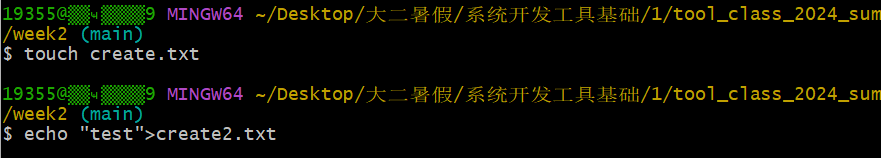
\includegraphics[width=1\textwidth]{create.png}\\
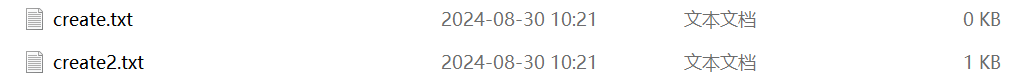
\includegraphics[width=1\textwidth]{create2.png}

\subsection{新建文件夹}
\subsubsection{新建单个文件夹:}
\begin{lstlisting}
    mkdir 文件夹名
\end{lstlisting}
\subsubsection{新建多个文件夹:}
\begin{lstlisting}
    mkdir 文件夹名1 文件夹名2 文件夹名3
\end{lstlisting}
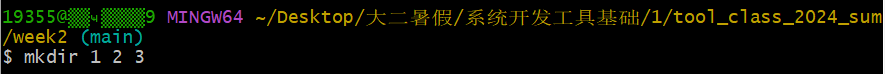
\includegraphics[width=1\textwidth]{./pictures/新建多个.png}\\
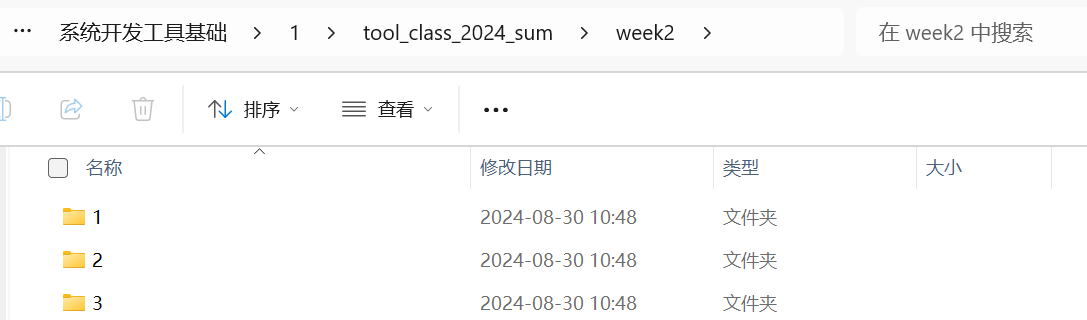
\includegraphics[width=1\textwidth]{./pictures/新建多个2.png}

\subsection{将命令一行一行写入脚本文件并执行}
用echo逐行添加命令,再用\verb|./semester|执行文件。\par
\textbf{注:>会覆盖文件内容,>>用于在文件末尾追加内容}\\
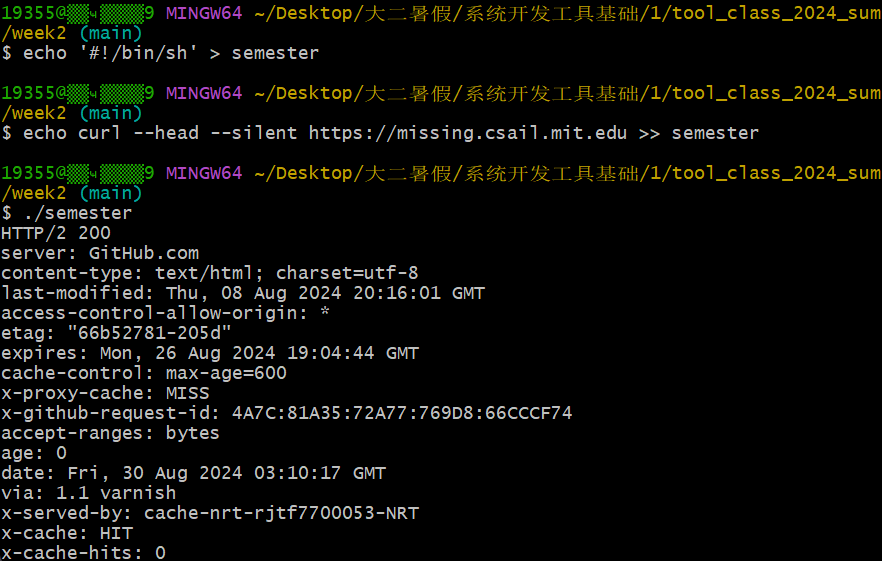
\includegraphics[width=1\textwidth]{./pictures/3.png}

\subsection{使用 | 和 > ,将 semester 文件输出的最后更改日期信息,写入当前目录下的 last-modified.txt 的文件中}
\subsubsection{管道操作符 |}
| 用于将左边的命令的输出内容传递给右边的命令
\subsubsection{行过滤工具 grep}
grep用于查找符合条件的行并输出\par
\verb|grep last-modified|\quad 可以查找有last-modified字样的行并输出
\subsubsection{实现}
\begin{center}
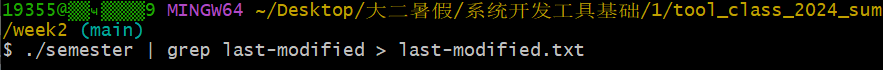
\includegraphics[width=1\textwidth]{./pictures/4.1.png}\\
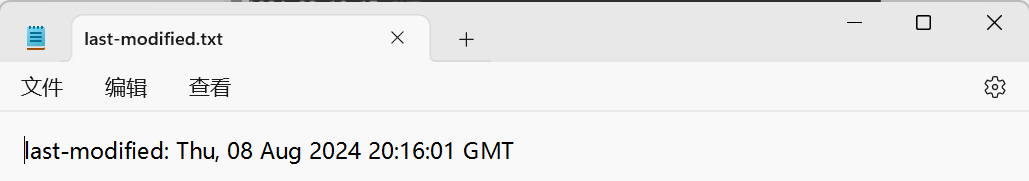
\includegraphics[width=1\textwidth]{./pictures/4.2.png}
\end{center}

\subsection{变量的输入输出}
\verb|read 变量名| \quad 可将用户输入内容赋值给变量\par
echo输出的字符串中用\verb|$name|表示变量\\
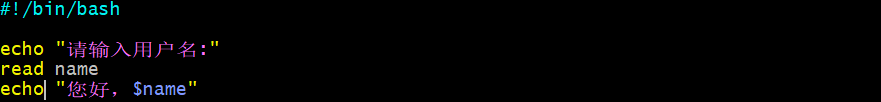
\includegraphics[width=1\textwidth]{./pictures/变量输入输出1.png}\par
\textbf{遇到的问题:}\par
一开始会报错\\
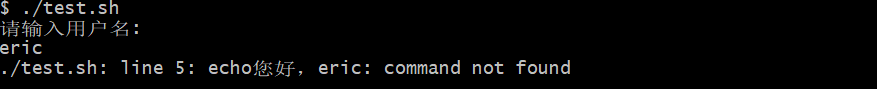
\includegraphics[width=1\textwidth]{./pictures/变量输入输出2.png}\par
原因:shell脚本中,命令和参数之间必须有空格。即echo和"输出的内容"间需有空格。
\subsection{猜字游戏}
\begin{lstlisting}
    #!/bin/bash

    number=$(shuf -i 1-10 -n 1)
    while [[ $num -ne $number ]] do
    echo "请输入1-10之间的数字"
    read num
    if [[ $num -eq $number ]];then
        echo "恭喜你猜对了"
    elif [[ $num -lt $number ]];then
        echo "猜小了"
    else
        echo "猜大了"
    fi
    done

\end{lstlisting}
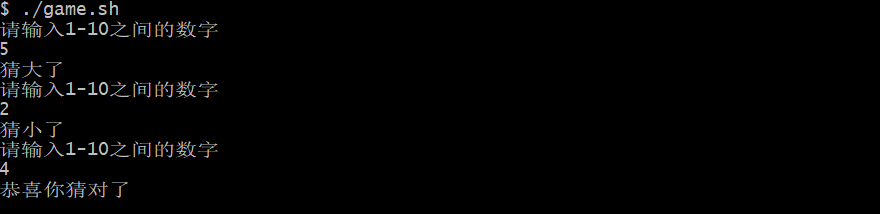
\includegraphics[width=1\textwidth]{./pictures/game.png}\par

\end{document}
